\documentclass[12pt, a4paper]{article}

\usepackage[UTF8]{ctex}
\usepackage{geometry}
\usepackage{graphicx}
\usepackage{float}
\usepackage{listings}
\usepackage{xcolor}
\usepackage{enumitem}

\geometry{left=2.5cm, right=2.5cm, top=3cm, bottom=3cm}

\lstset{
    language=Python,
    basicstyle=\small\ttfamily,
    keywordstyle=\color{blue},
    stringstyle=\color{red},
    commentstyle=\color{green!50!black},
    showstringspaces=false,
    breaklines=true,
    frame=single,
    numbers=left,
    numberstyle=\tiny\color{gray}
}

\setlength{\parindent}{0pt}

\begin{document}

\begin{center}
    {\LARGE \textbf{计算机视觉实验报告} \\[1.5cm]}
    {\large \textbf{实验 10}} \\[0.8cm]
    {\large 姓名：周梓俊} \\[0.4cm]
    {\large 学号：23120899} \\[1.1cm]
\end{center}

\textbf{题目 1}

\begin{enumerate}[label=\textbf{\alph*)}, leftmargin=*]

\item \textbf{程序代码}

\begin{lstlisting}
class SimpleCNN(nn.Module):
    def __init__(self) -> None:
        super().__init__()
        self.features = nn.Sequential(
            nn.Conv2d(1, 32, kernel_size=3, padding=1),
            nn.ReLU(inplace=True),
            nn.MaxPool2d(kernel_size=2, stride=2),
            nn.Conv2d(32, 64, kernel_size=3, padding=1),
            nn.ReLU(inplace=True),
            nn.MaxPool2d(kernel_size=2, stride=2),
        )
        self.classifier = nn.Sequential(
            nn.Flatten(),
            nn.Linear(64 * 7 * 7, 128),
            nn.ReLU(inplace=True),
            nn.Dropout(p=0.2),
            nn.Linear(128, 10),
        )

    def forward(self, x):
        x = self.features(x)
        x = self.classifier(x)
        return x

transform = transforms.Compose([
    transforms.ToTensor(),
    transforms.Normalize((0.1307,), (0.3081,))
])

train_dataset = datasets.MNIST(root=data_dir, train=True, download=True, transform=transform)
test_dataset = datasets.MNIST(root=data_dir, train=False, download=True, transform=transform)

optimizer = torch.optim.Adam(model.parameters(), lr=0.001)
criterion = nn.CrossEntropyLoss()
\end{lstlisting}

\item \textbf{实验结果截图}

\begin{figure}[H]
    \centering
    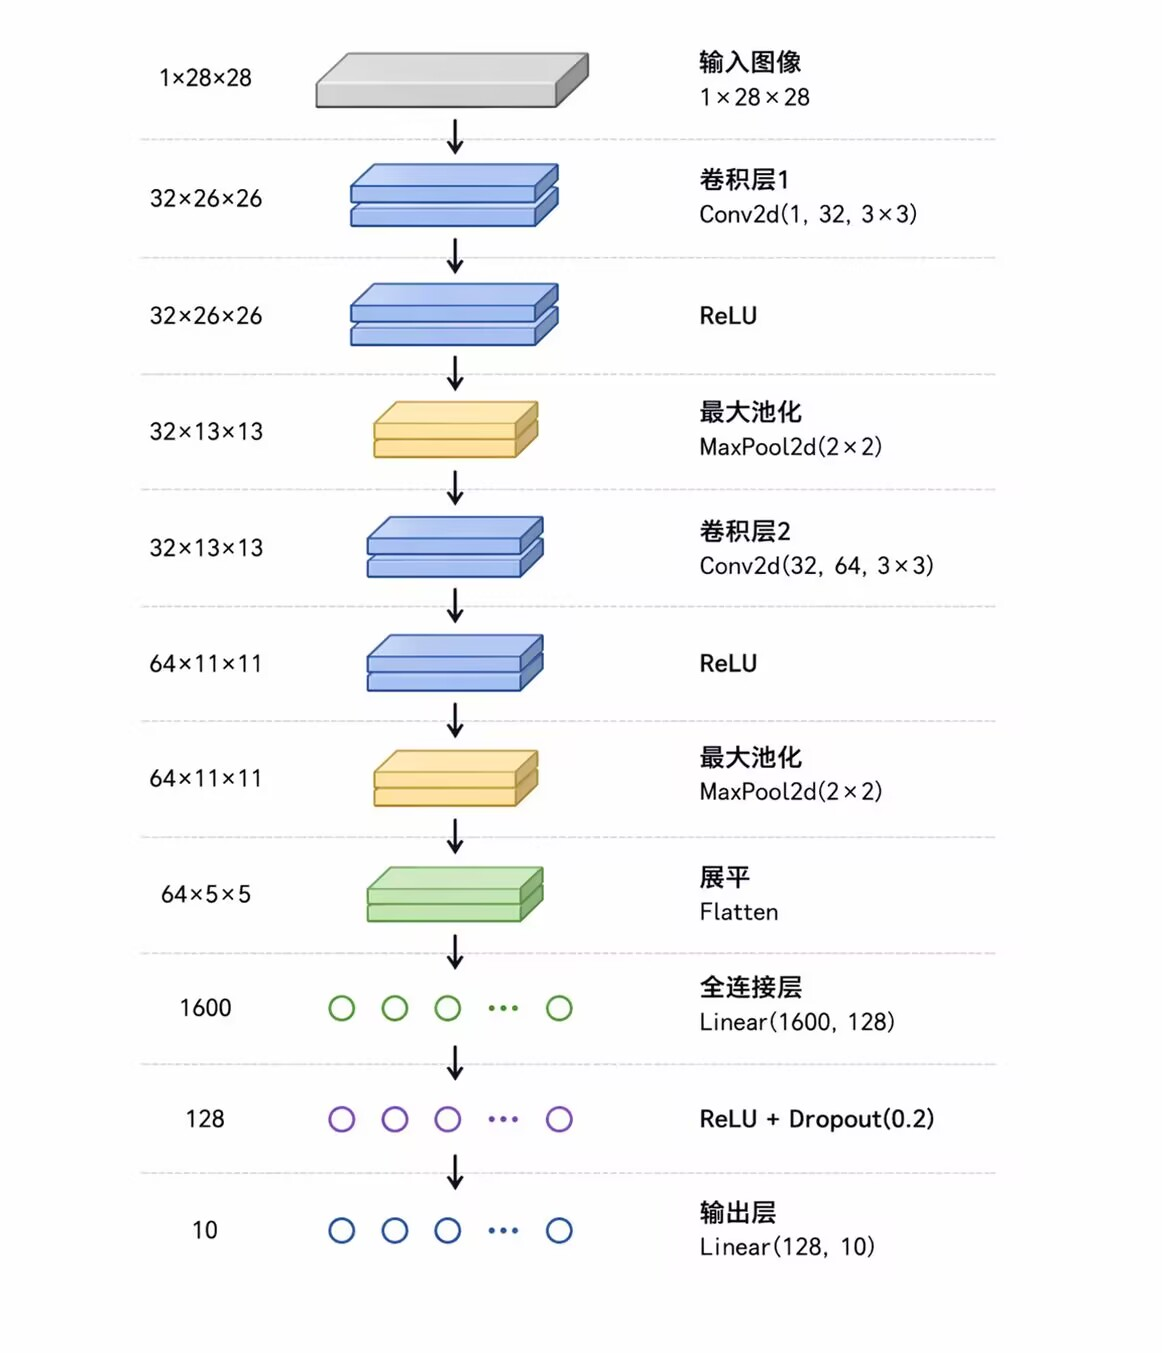
\includegraphics[width=0.50\textwidth]{outputs/cnn_structure.jpg}
    \\[4pt]{\small CNN 网络结构示意图}
\end{figure}

\begin{figure}[H]
    \centering
    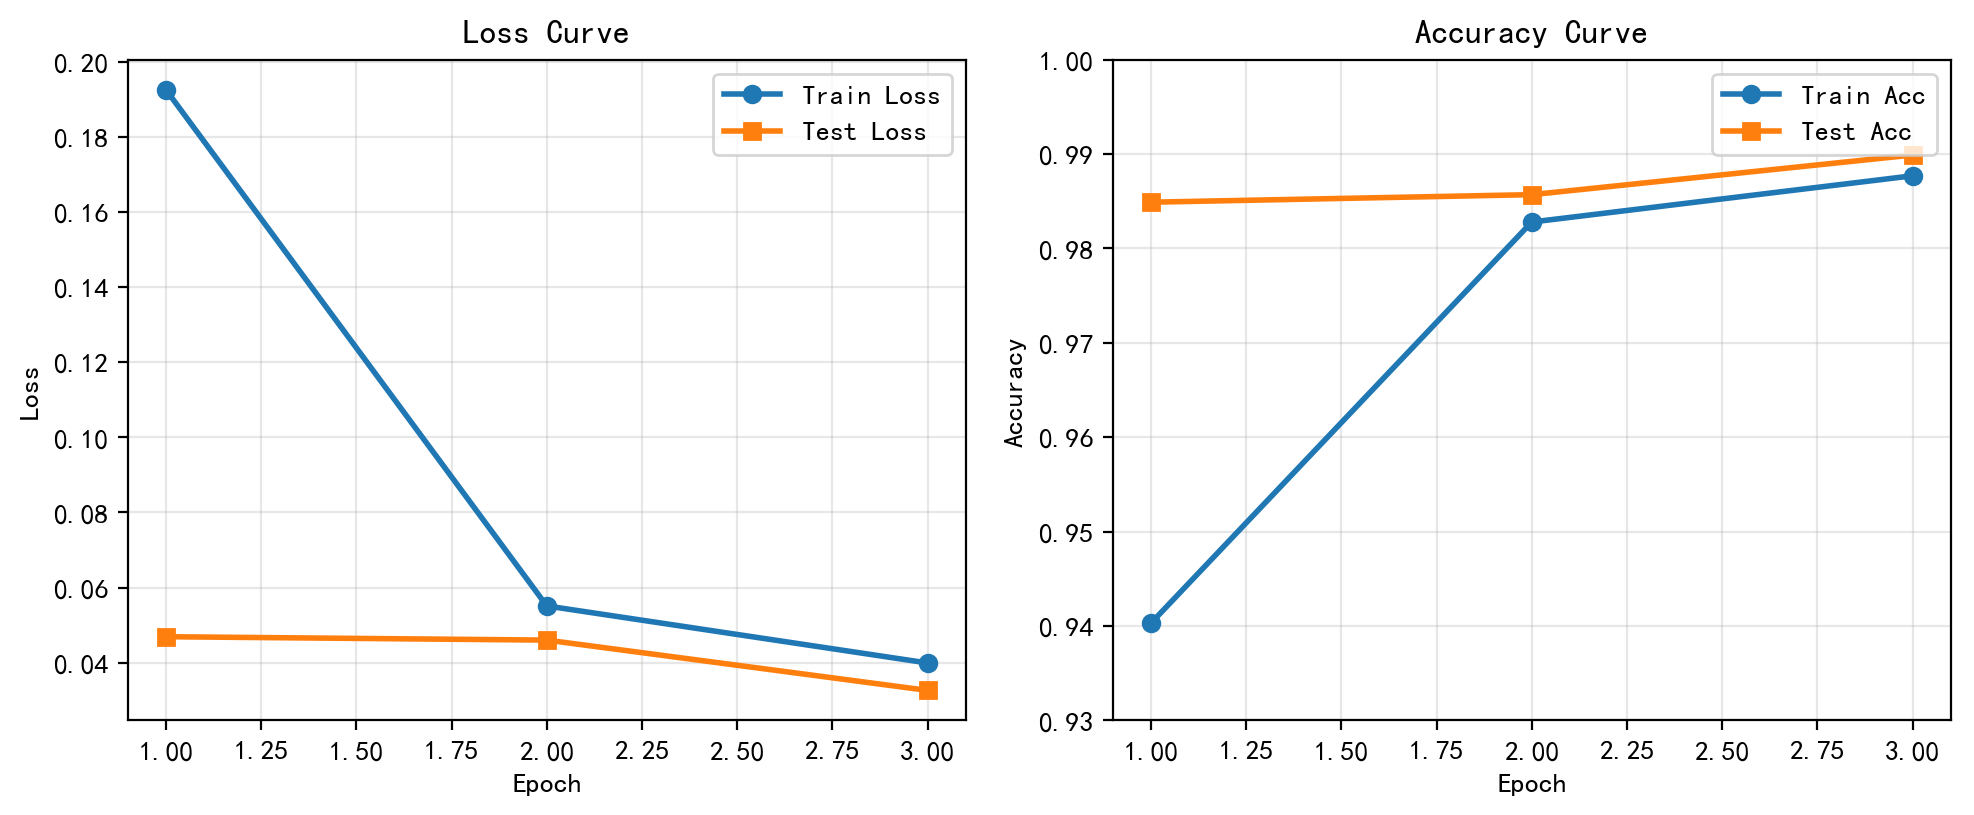
\includegraphics[width=0.78\textwidth]{outputs/training_curves.png}
    \\[4pt]{\small 训练损失与准确率曲线}
\end{figure}

\begin{figure}[H]
    \centering
    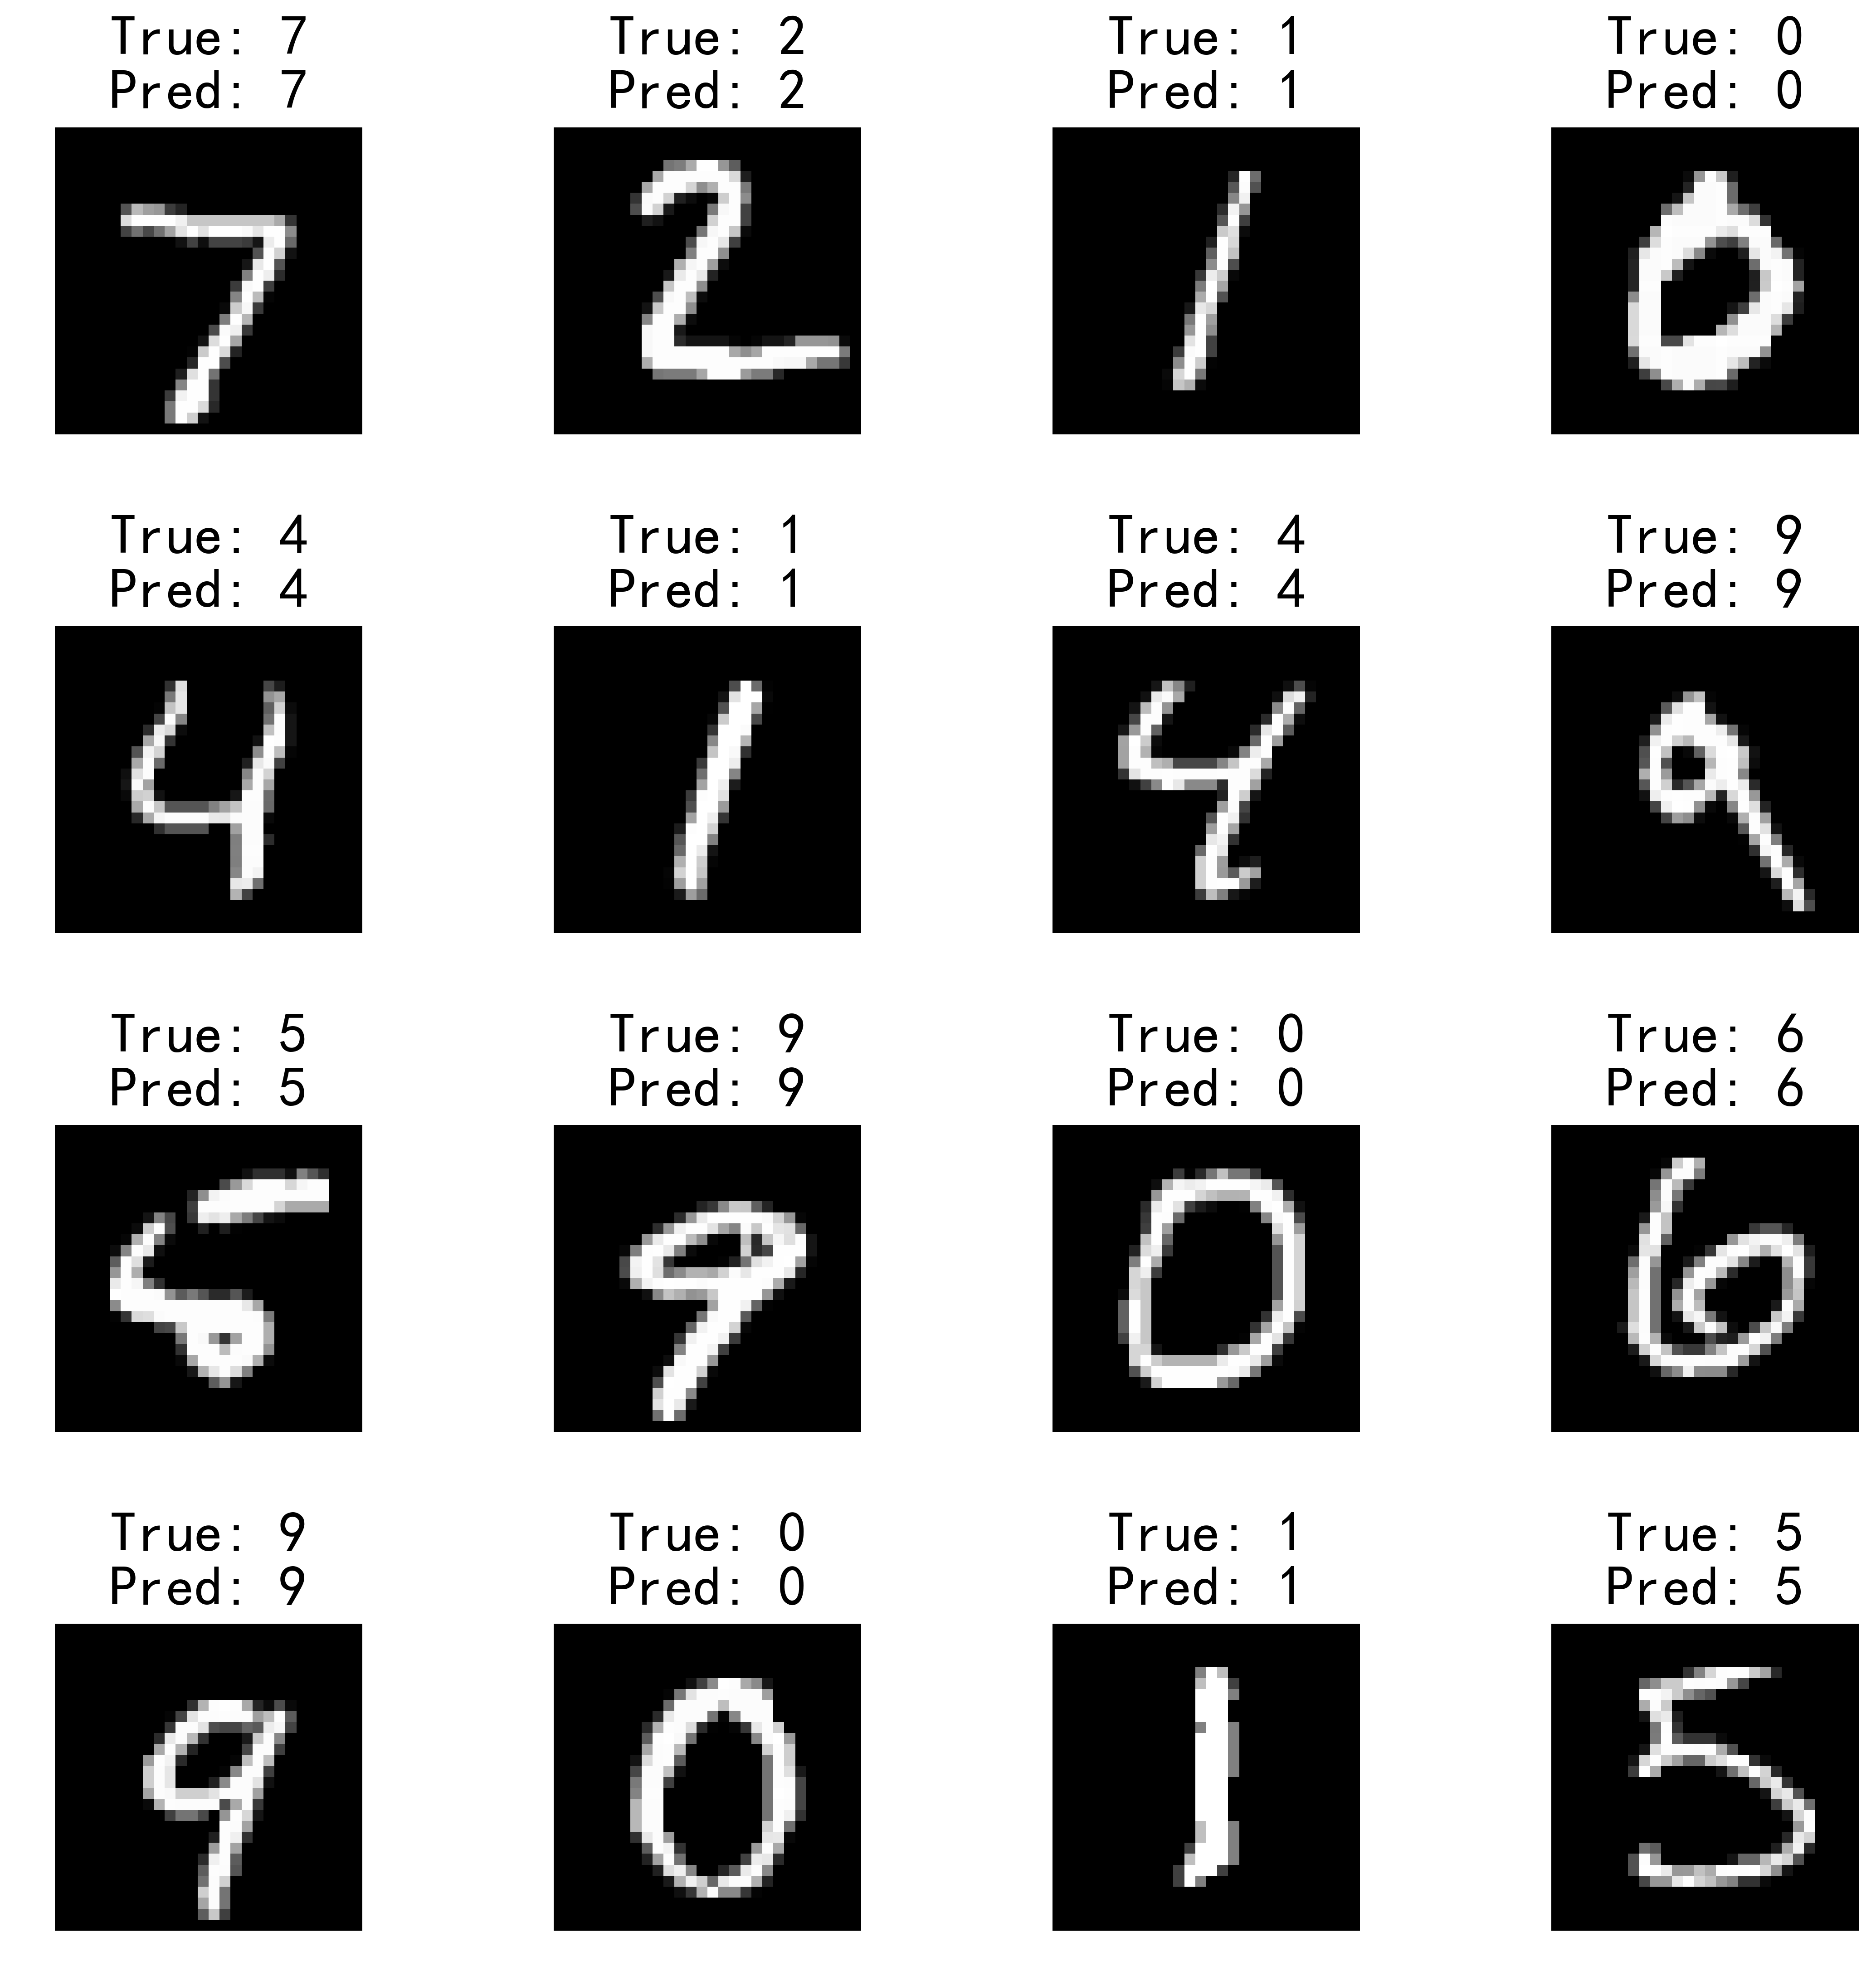
\includegraphics[width=0.82\textwidth]{outputs/sample_predictions.png}
    \\[2pt]{\small 测试样本预测结果}
\end{figure}

\begin{figure}[H]
    \centering
    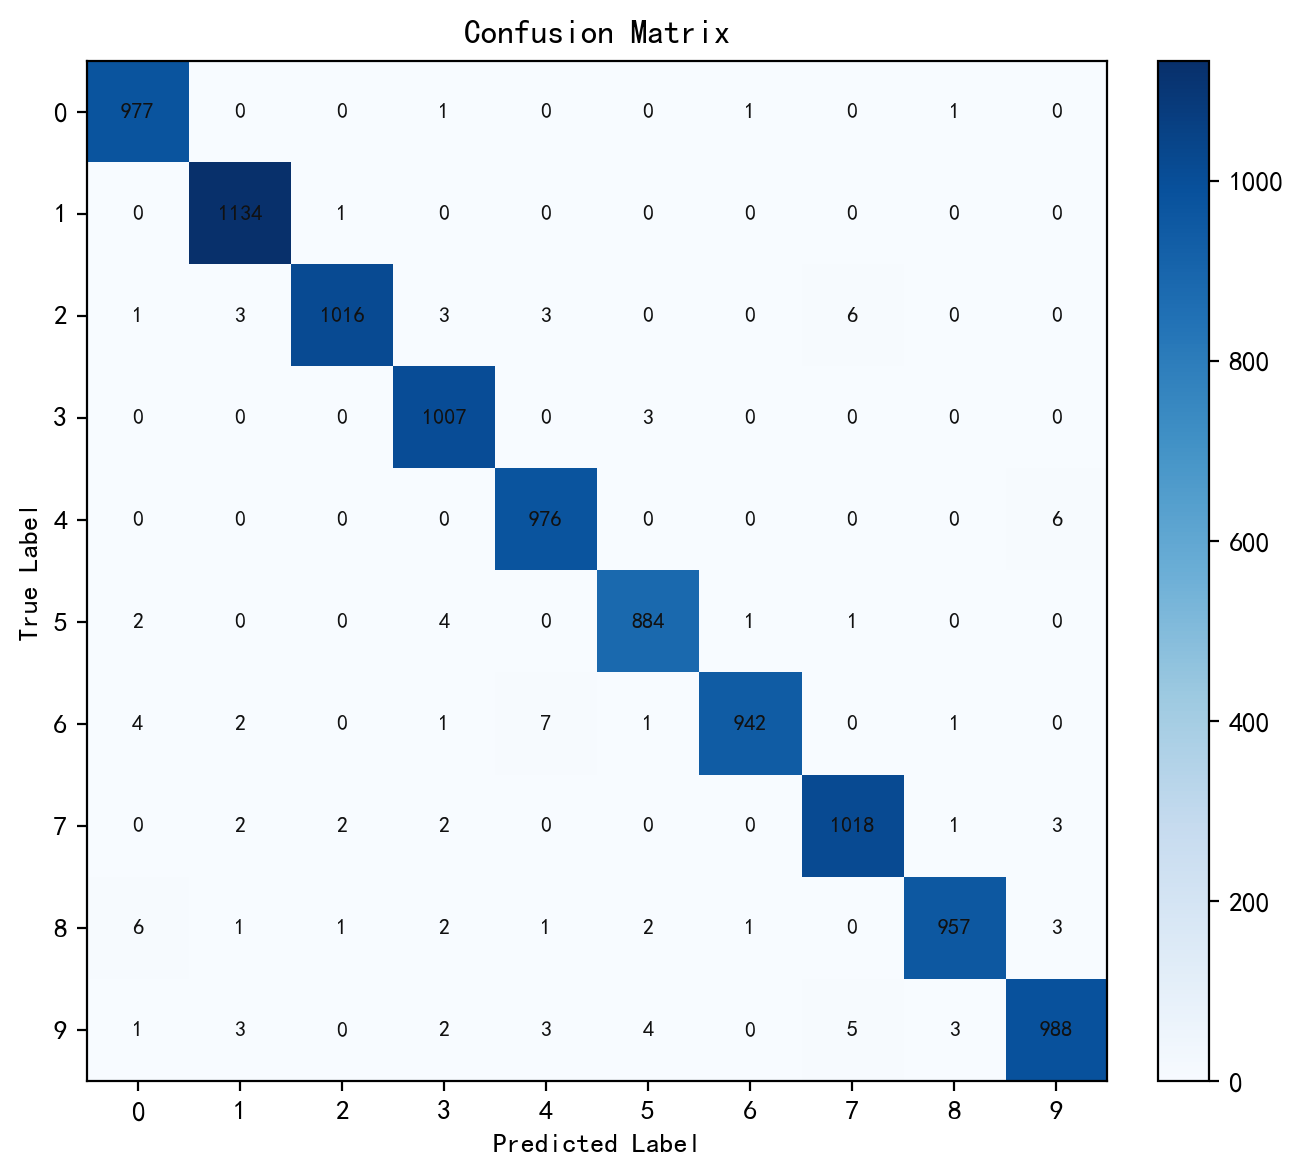
\includegraphics[width=0.62\textwidth]{outputs/confusion_matrix.png}
    \\[2pt]{\small 测试集混淆矩阵}
\end{figure}

\item \textbf{结果分析}

本实验使用 PyTorch 实现卷积神经网络，数据集采用 MNIST 手写数字数据集，其中训练集 60000 张，测试集 10000 张，图像大小为 $28 \times 28$。网络由两层卷积层、两层最大池化层和两层全连接层组成，能够完成 0 到 9 共 10 类手写数字识别任务。

从训练曲线可以看出，随着 epoch 增加，训练损失和测试损失逐渐下降，训练准确率和测试准确率逐渐上升，说明模型训练过程稳定且收敛较好。3 个 epoch 训练结束后，模型在测试集上的最终准确率达到 98.99\%，表明该卷积神经网络能够较好完成 MNIST 手写数字识别任务。

从测试样本预测结果和混淆矩阵可以看出，大多数数字都能被正确分类，只有少量形状相近的数字存在误判。这说明卷积神经网络能够有效提取图像中的局部特征，对基础图像分类任务具有较好的识别效果。

\end{enumerate}

\end{document}
